\documentclass[12pt,a4paper,openright,twoside]{book}
\usepackage[utf8]{inputenc}
\usepackage{disi-thesis}
\usepackage{code-lstlistings}
\usepackage{notes}
\usepackage{shortcuts}
\usepackage{acronym}
\usepackage[acronym]{glossaries}

\school{\unibo}
\programme{Corso di Laurea Triennale in Ingegneria e Scienze Informatiche}
\title{DGA Domain Generation Algorithm}
\author{Simone Collorà}
\date{\today}
\subject{Programmazione a Oggetti}
\supervisor{Prof. Mirko Viroli}
\cosupervisor{Dott. CoSupervisor 1}
\morecosupervisor{Dott. CoSupervisor 2}
\session{I}
\academicyear{2024-2025}

% Definition of acronyms
\acrodef{IoT}{Internet of Thing}
\acrodef{vm}[VM]{Virtual Machine}
\newacronym{DGA}{DGA}{Domain Generation Algorithm}
\newacronym{C&C}{C\&C}{Command and Control}
\newacronym{P2P}{P2P}{Peer to Peer}


\mainlinespacing{1.241} % line spacing in mainmatter, comment to default (1)

\begin{document}
\frontmatter\frontispiece
\nocite{*}

\begin{abstract}	
Max 2000 characters, strict.
\end{abstract}

\begin{dedication} % this is optional
Optional. Max a few lines.
\end{dedication}

%----------------------------------------------------------------------------------------
\tableofcontents   
\listoffigures     % (optional) comment if empty
\lstlistoflistings % (optional) comment if empty
%----------------------------------------------------------------------------------------

\mainmatter

%----------------------------------------------------------------------------------------
\chapter{Introduction}
\label{chap:introduction}
%----------------------------------------------------------------------------------------

Write your intro here.
%\sidenote{Add sidenotes in this way. They are named after the author of the thesis}

La sicurezza informatica è un argomento di crescente importanza
nel mondo moderno. Con il passare del tempo,
i sistemi di protezione sono diventati sempre più sofisticati
e potenti ma, allo stesso tempo, anche gli hackers 
hanno sviluppato tecniche sempre più avanzate per eludere i sistemi di protezione.
Tra queste vi è sicuramente l'uso di Botnets
dei \acrfull{C&C} servers. I \acrshort{C&C} sono dei server che manipolano
i computer infetti da malwares, i Botnets, permettendo
all'attaccante di eseguire codice malevolo da remoto.
Il malware, però, deve conoscere un indirizzo IP o un dominio
per contattare il server. L'attaccante potrebbe
inserire in modo bruto l'indirizzo IP del server nel codice del malware,
ma questo metodo è facilmente rilevabile e bloccabile.
Gli hackers, quindi, preferiscono utilizzare dei domini
generati in modo pseudo casuale per nascondere i loro server chiamati
\acrfull{DGA} servers.



\paragraph{Structure of the Thesis}

%\note{At the end, describe the structure of the paper}

\chapter{Uso di Machine Learning e AI per rilevare i DGA}

\section{Botnets e C\&C}
I suggest referencing stuff as follows: \cref{fig:DGA example} or \Cref{fig:DGA example}

\subsection{Botnets}

I Botnets sono reti di computer infetti da malware, chiamati bot,
che possono essere controllati da un attaccante, il botmaster.
La vita di un botnet di solito sono questi:
\begin{enumerate}
    \item \textbf{Infezione e propagazione}: Questo è il primo
    passaggio. L'attaccante cerca di infettare un computer
    tramite vari metodi come email con link malevoli o \acrfull{P2P} sharing.
    Una volta infettato un dispositivo, il malware cerca di infettare
    altri dispositivi nella rete.

    \item \textbf{Rallying}: i bots cercano di contattare per la prima volta
    il server \acrshort{C&C} per far capire all'attaccante
    che l'attacco è andato a buon fine.

    \item \textbf{Commands and Reports}: il malware esegue le istruzioni
    ricevute dal server \acrshort{C&C} e invia i risultati al botmaster.
    I bots ascoltano i comandi dal server \acrshort{C&C} 
    o si connettono ad esso periodicamente. Appena ricevono
    un comando lo eseguono, inviano i risultati al botmaster
    e aspettano un nuovo comando.

    \item \textbf{Abbandono}: Quando un bot non è più utile o utilizzabile,
    il botmaster può decidere di abbandonarlo. Il botnet, invece,
    sarà completamente distrutto quando tutti i bot saranno
    abbandonati o bloccati dalla vittima o quando il \acrshort{C&C} server
    verrà bloccato


\end{enumerate}

\begin{figure}
    \centering
    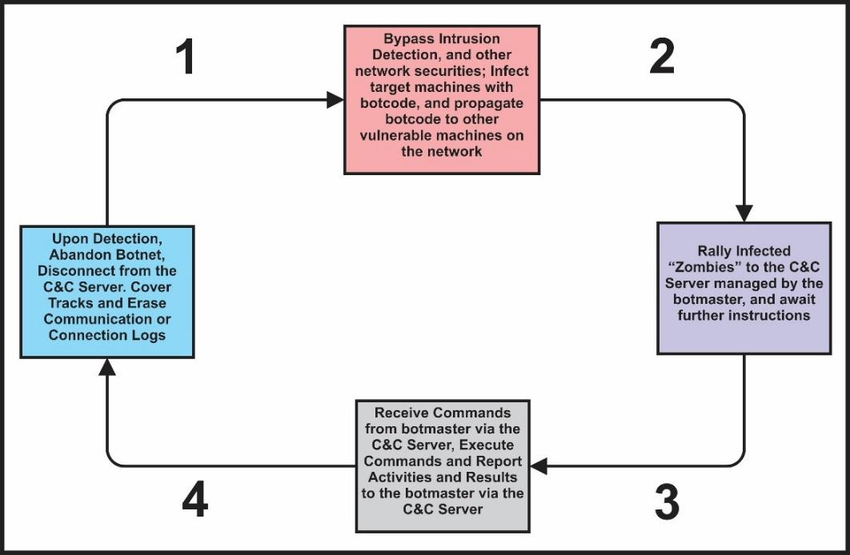
\includegraphics[width=.8\linewidth]{figures/The-Lifecycle-Schema-of-a-typical-Botnet.png}
    \caption{Ciclo di vita di un botnet (da \cite{Ogu2016})}
    \label{fig:botnet}
\end{figure}

\subsection{C\&C}




% \begin{image}
%     \centering
%     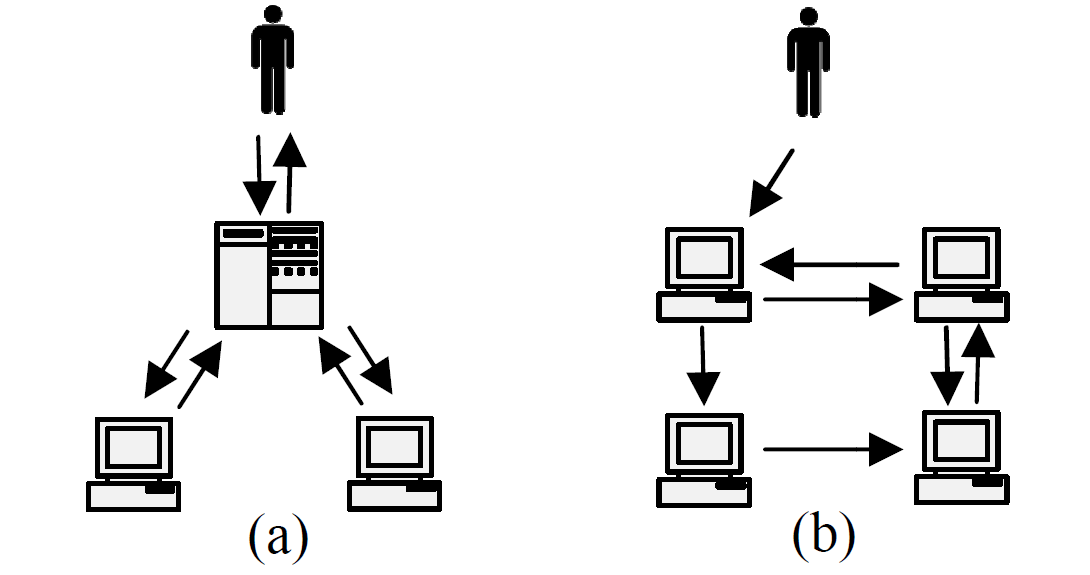
\includegraphics[width=.8\linewidth]{figures/Types-of-CC.png}
%     \caption{Tipi di server \acrshort{C\&C} (a) centralizzati, (b) decentralizzati}
%     \label{fig:command and control}
% \end{image}


I \acrshort{DGA} sono algoritmi che generano migliaia di domini in modo pseudo casuale.
Prima viene scelto un seed, di solito la data odierna
o anche le previsioni meteo \cite{8621875} e, tramite
un algoritmo di hashing, vengono generati i domini.
Questi domini vengono poi utilizzati per contattare i server \acrshort{C&C}.
Non tutti i domini generati però sono registrati.
Il computer infetto, tramite i DNS locali, cercherà di tradurre
un dominio in un indirizzo IP.
Se non riesce a contattarlo con un determinato dominio,
proverà con il successivo finché non troverà
un dominio valido che permetterà al malware di comunicare con
il server \acrshort{C&C} \cite{8489147}.
In questo modo, diventa più difficile per i sistemi di protezione
rilevare e bloccare i loro attacchi.
Si potrebbe pensare di bloccare direttamente i domini tramite
una blacklist ma questo metodo
risulta inefficace poiché vengono generati migliaia di domini
continuamente. Si pensi che Conficker C, un famoso malware
che utilizza \acrshort{DGA}, è in grado di generare
fino a 50.000 domini pseudo casuali al giorno \cite{978131}.

Un altro modo per contrastare ciò
potrebbe essere quello di fare reverse engineering
del \acrshort{DGA} per capire quale seed viene utilizzato per generare i domini.
Questo però risulta lento e dispendioso e possibilmente inefficace \cite{8887881}.

\begin{figure}
    \centering
    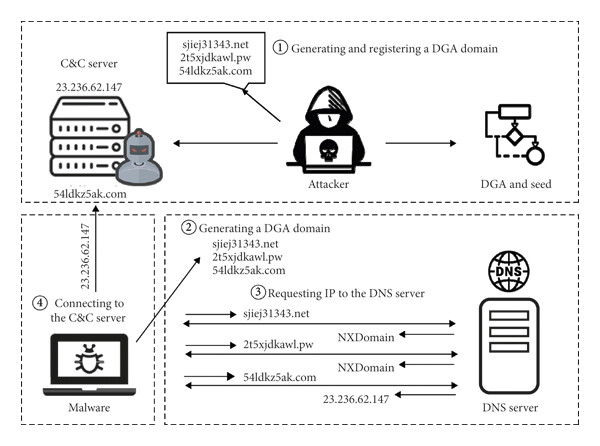
\includegraphics[width=.8\linewidth]{figures/DGA example.jpg}
    \caption{esempio del funzionamento di un \acrshort{DGA}}
    \label{fig:DGA example}
\end{figure}

Per contrastare i \acrshort{DGA}, sono stati sviluppati
vari metodi di machine learning in grado di rilevare i domini generati.
Questi metodi hanno due lati poisitivi:
\begin{itemize}
    \item Non richiedono un lungo processo di reverse engineering.
    \item Essendo l'AI una blackbox, è molto difficile
    per gli hackers eseguire un reverse engineering del modello.
\end{itemize}






\section{Some cool topic}

\chapter{Contribution}

You may also put some code snippet (which is NOT float by default), eg: \cref{lst:random-code}.

\lstinputlisting[float,language=Java,label={lst:random-code}]{listings/HelloWorld.java}

\section{Fancy formulas here}

%----------------------------------------------------------------------------------------
% BIBLIOGRAPHY
%----------------------------------------------------------------------------------------

\backmatter

\bibliographystyle{IEEEtran} %prima era alpha
\bibliography{bibliography}

\begin{acknowledgements} % this is optional
Optional. Max 1 page.
\end{acknowledgements}

\end{document}
